\section{Implementierung mit Xamarin}
In diesem Abschnitt wird die Implementierung der N��ing ScanApp mit Xamarin.Forms beschrieben. 
Es wurde das f�r Xamarin �bliche MVVM-Muster angewendet.\\Bei Xamarin.Forms gibt es zwei alternative
Methoden zum Code-Sharing:
 Shared Projects und Portable Class Libraries (PCL). Da im vorliegenden Fall Code-Sharing nur
 innerhalb der N��ing App vorgesehen wurde, wurde Shared Projects gew�hlt (der PCL
 Ansatz wird f�r den Fall empfohlen, wenn der Entwickler seinen Code f�r andere Developer in Form einer DLL Bibliothek bereitstellen m�chte).
Beim Erstellen des Xamarin.Forms Projekts namens ScanApp wurden automatisch zwei weitere Projekte
erstellt, so dass folgende Projekte entstanden sind:
\begin{itemize}
  \item ScanApp - das gemeinsame Projekt. Hier wird die Gesch�ftslogik der Anwendung implementiert.
  \item ScanApp.Droid - plattformspezifisches Projekt f�r Android.
  \item ScanApp.iOS - plattformspezifisches Projekt f�r iOS.
\end{itemize}
\subsection{Persistierung der Daten SQLite}
F�r die Persistenz der Appdaten wurde die open-source Datenbank SQLite eingesetzt.\\SQLite ist gut
geeignet f�r Cross-Plattform-Entwicklung, weil:
\begin{itemize}
  \item die Datenbank klein, schnell und leicht portierbar ist;
  \item der Fileformat leicht zu benutzen und plattform�bergreifend ist;
  \item SQLite die meisten SQL92 Standards implementiert.
\end{itemize}
Da
beim gemeinsamen ScanApp Projekt keine Bibliotheken eingebunden werden k�nnen, muss man einen
SQLite.cs File aus Github herunterladen und in das gemeinsame Projekt kopieren. Dieser C\#-File
benutzt Compiler Direktiven um mehrere Plattformen in derselben Codebasis zu unterst�tzen.
\\Um SQLite in einer Xamarin.iOS oder Android Applikation benutzen zu k�nnen, muss man angeben, wo
der Datenbank File zu finden ist (es ist abh�ngig vom
Ziel-Plattform unterschiedlich). F�r iOs und Android kann man Environment class benutzen um einen
validen Pfad zu konstruieren (siehe Abb. \ref{fig:abb27}). Mittels Compiler Direktiven lassen sich
spezielle Pfade f�r jede Plattform generieren.\\Um sicher zu gehen, dass der Code nicht versucht,
auf die SQLite Datenbank aus verschiedenen multiple Threads zuzugreifen wird manuel ein "`lock"'
benutzt. Z.B.\\object locker = new object();\\lock(locker)\{ Datenbankquery \};\\Alle
Datenbankzugriffe sind mit demselben "`lock"' gekapselt.
\begin{figure}[!h]
\centering
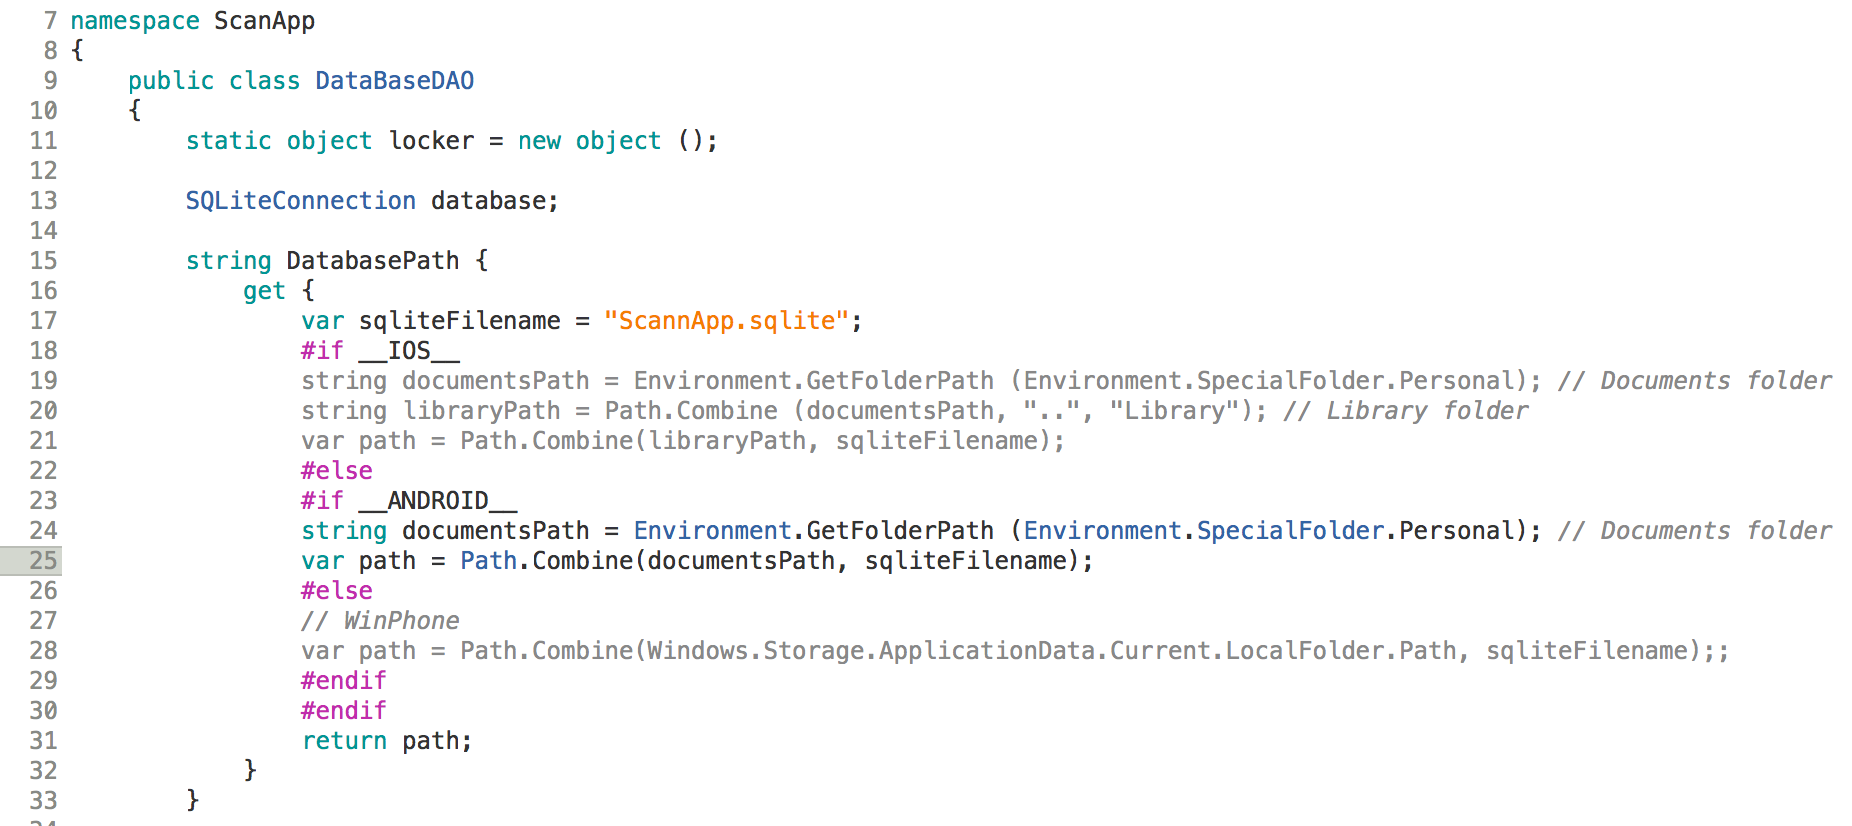
\includegraphics[scale = 0.4]{graphics/SQLitePath.png}
\caption{SQLite Pfad}
\label{fig:abb27}
\end{figure}

\subsection{GUI}
Die Benutzeroberfl�chen werden mit wenigen Ausnahmen im gemeinsamen Projekt, ScanApp erstellt.
Xamarin l�sst Entwicklern die Wahl zwischen der Markupsprache Xaml und C\# f�r die Implementierung
der UIs (User Interfaces).\\Mit C\# lassen sich die Positionierung der Steuerelemente und deren
Funktionalit�t in einer C\#-Datei implementieren, aber das macht den Code schwer lesbar und nicht
wiederverwendbar. Aus diesem Grund wurden die grafischen Interfaces der N��ing ScanApp mit der
Markupsprache Xaml beschrieben.
Somit wurde eine strikte Trennung zwischen dem Oberfl�chendesign (in einer
Xaml-Datei beschrieben) und der Funktionalit�t (in der
zugrundeliegenden (Code-Behind) C\#-Datei implementiert) erreicht. Dar�ber hinaus gibt Xaml die
M�glichkeit, dass Designer und Entwickler unabh�ngig voneinander arbeiten k�nnen.\\Bei der
Erstellung einer Xamarin.Forms ContentPage Xaml-Datei wird automatisch auch die zugrundeliegende C\#-Datei, sogenannte Code-Behind-Datei, angelegt (siehe Abb. \ref{fig:abb21}).

 In Abbildung \ref{fig:abb23} sieht man den Xaml-Code f�r die Benutzeroberfl�che, die in Abbildung
\ref{fig:abb24} zu sehen ist. Der Aufbau einer Xaml-Datei entspricht eines XML-Dokuments. Es gibt ein Wurzelelement und jedes
Element kann Attribute besitzen. Dadurch entsteht eine �bersichtliche Hierarchie der Elemente. Durch
das Attribut x:Name kann man auf das Element aus dem Code-Behind-Datei zugreifen und so kann man
z.B. den Text eines Labels oder die Textfarbe �ndern (siehe \ref{fig:abb26}).
\\In Abbildung \ref{fig:abb25} sieht man die zugrundeliegenden C\#-Datei, in der z.B. die
Funktionalit�t der Toolbar-Buttons implementiert ist. Beim Klick auf den Button zum Speichern der
Angaben, werden die Texten der Texteingabefeldern in einem Objekt vom Typ Kopfdaten gespeichert und
anschlie�end wird das neu erstellte Objekt in die SQLite-Datenbank gespeichert. Beim Klick auf den
M�llkorb-Button, werden die gespeicherten pers�nlichen Daten aus der SQLite-Datenbank gel�scht. 
\begin{figure}[!h]
\centering

\includegraphics[scale = 0.7]{graphics/XamlDateiPlusCSDatei.png}
\caption{Xaml-Datei und die zugrundeliegende C\#-Datei}
\label{fig:abb21}
\end{figure}

\begin{figure}[!h]
\centering
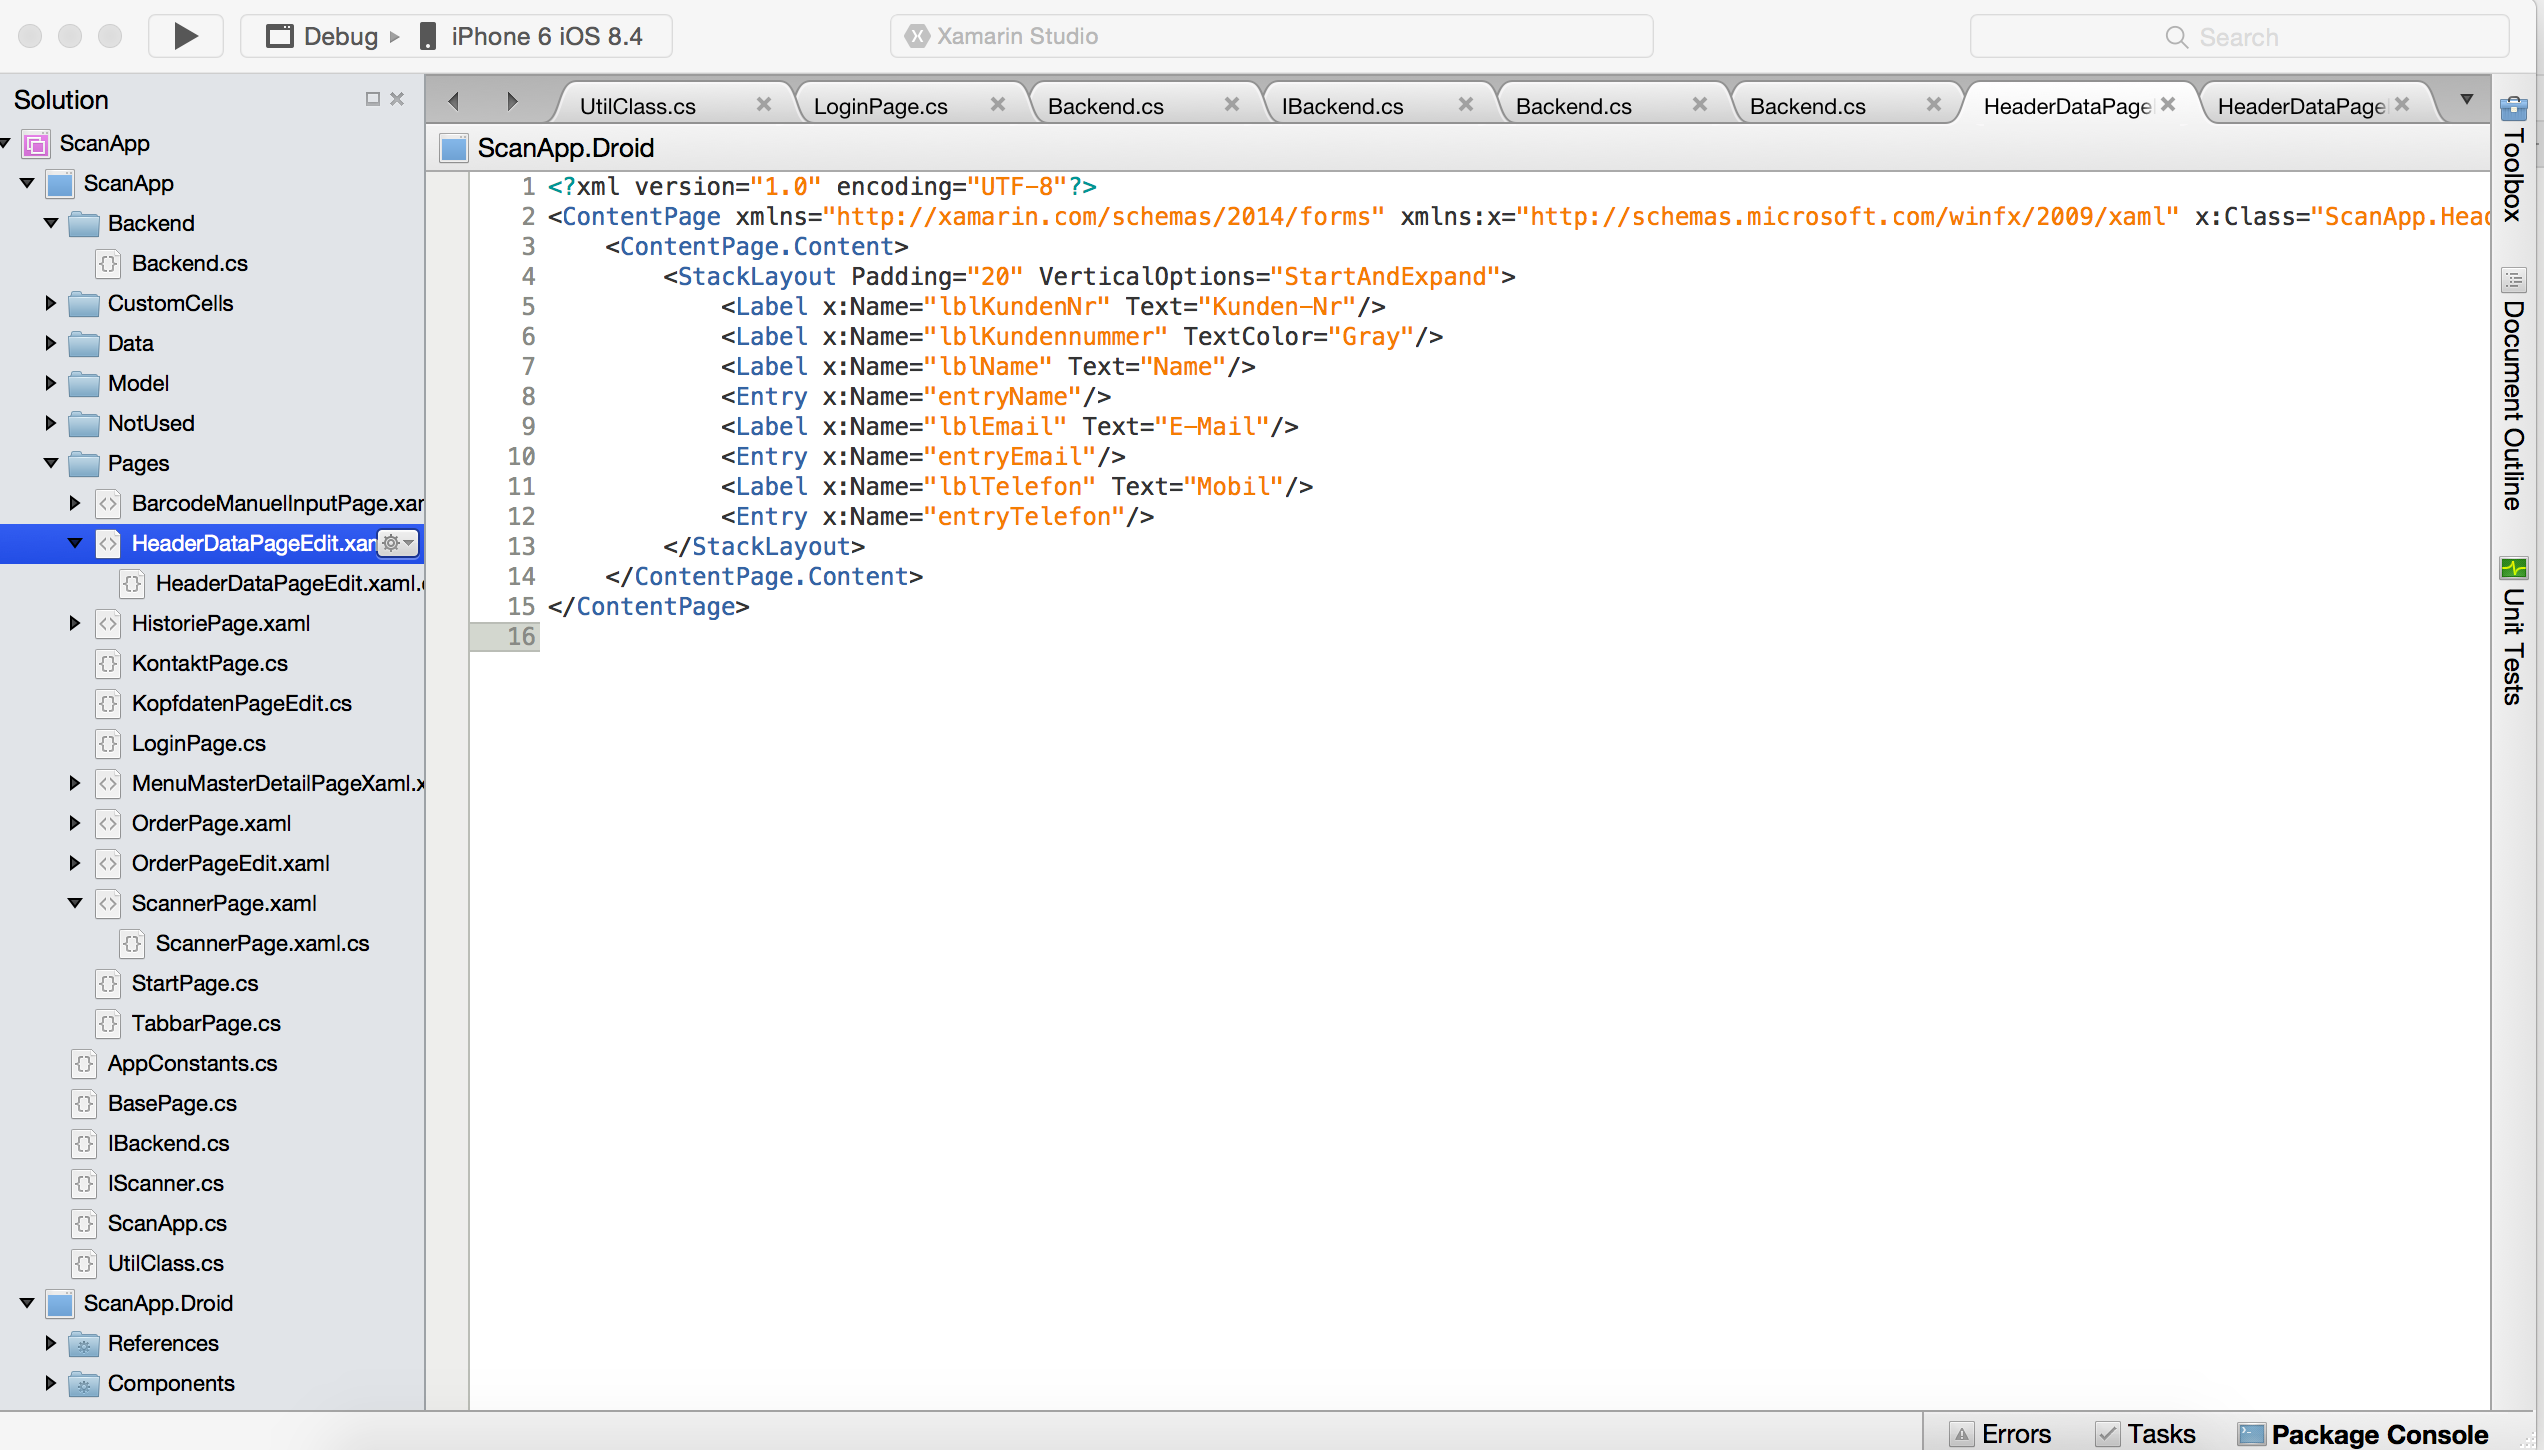
\includegraphics[scale = 0.324]{graphics/XamlDatei.png}
\caption{Xaml-Datei}
\label{fig:abb23}
\end{figure}
\begin{figure}[!h]
\centering
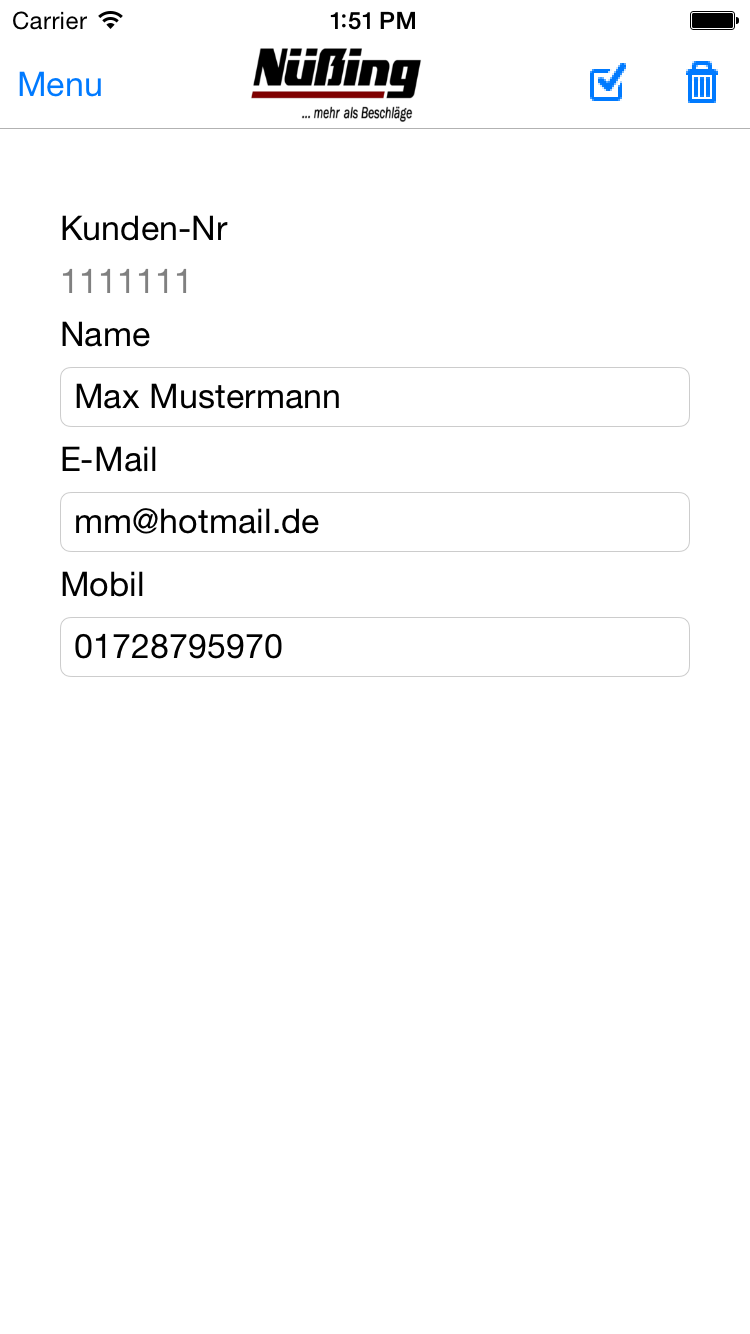
\includegraphics[scale = 0.3]{graphics/appScreenshots/PersoenlicheDaten.png}
\caption{Screenshot: Seite zum Editieren der pers�nlichen Daten eines Nutzers der ScanApp}
\label{fig:abb24}
\end{figure}
\begin{figure}[!h]
\centering
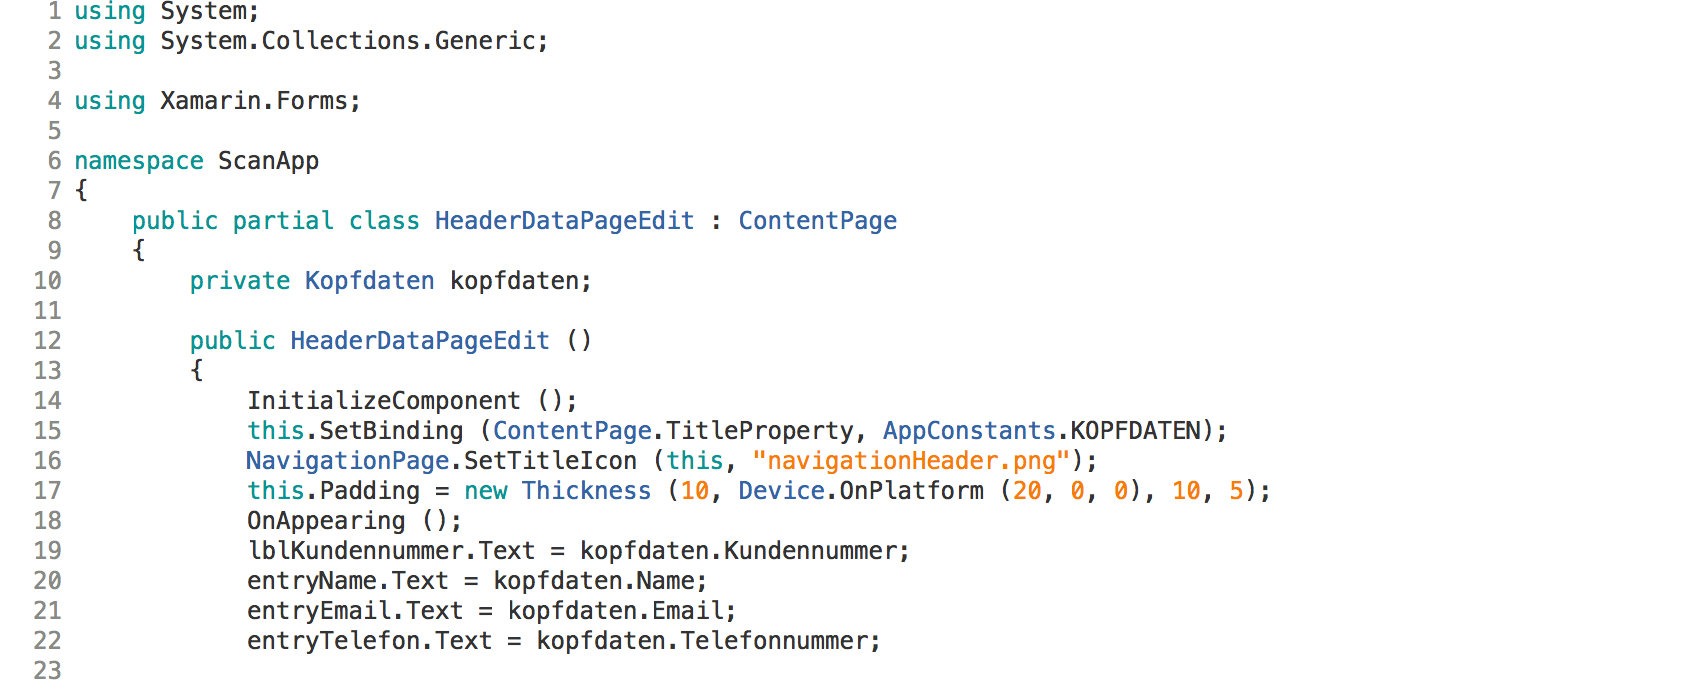
\includegraphics[scale = 0.4]{graphics/HeaderDatenCSDatei.png}
\caption{Zugrundeliegende (Code-Behind) C\#-Datei}
\label{fig:abb26}
\end{figure}
\begin{figure}[!h]
\centering
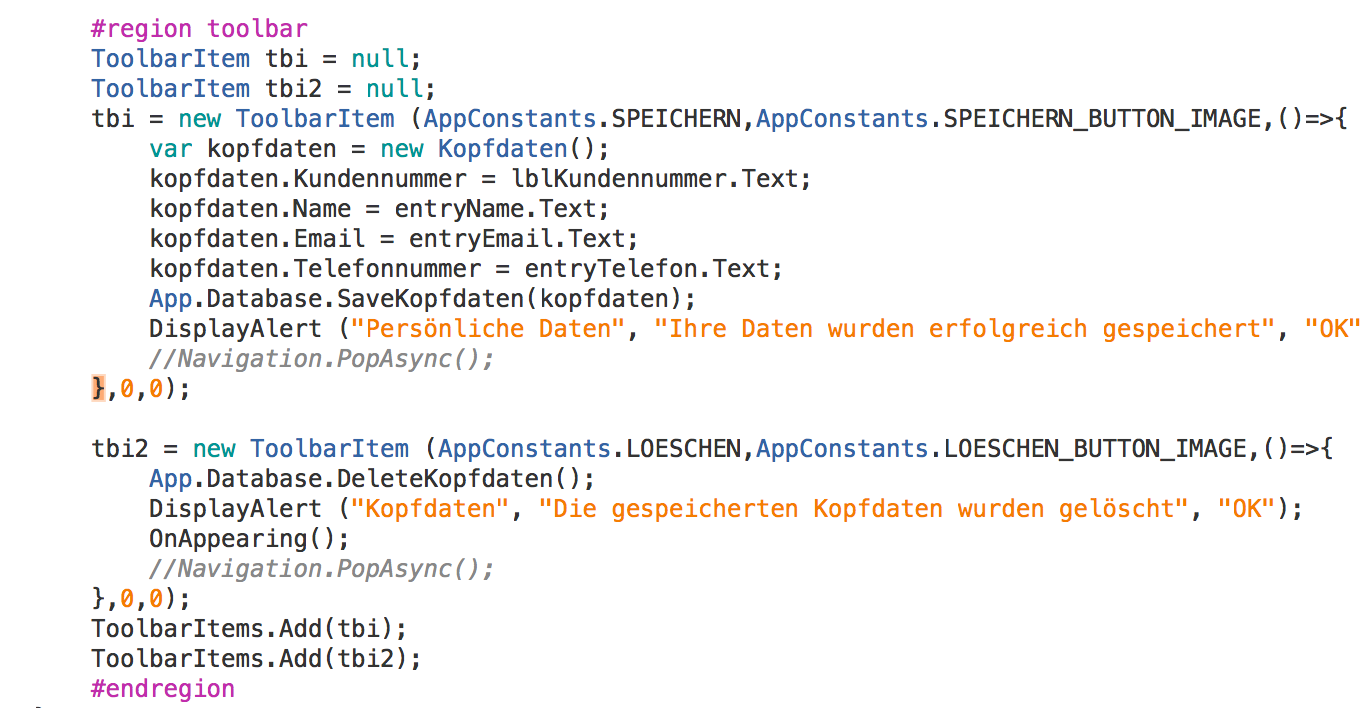
\includegraphics[scale = 0.5]{graphics/HeaderDatenToolbar.png}
\caption{Zugrundeliegende C\#-Datei}
\label{fig:abb25}
\end{figure}

\subsection{Implementierung des Barcodescanners}
Die Implementierung des Barcodescanners ist einer der wenigen Punkten, bei denen man auf die
plattformspezifischen Projekte zugreifen musste. In beiden plattformspezifischen Projekte musste die
Komponente ZXing.Net.Mobile hinzugef�gt werden. Im gemeinsamen Projekt wurde das Interface
IScanner.cs
erstellt (Abb. \ref{fig:abb28}). In beiden plattformspezifischen Projekte wurde je eine Klasse
Scanner.cs erstellt, die dieses Interface implementiert. 
\begin{figure}[!h]
\centering
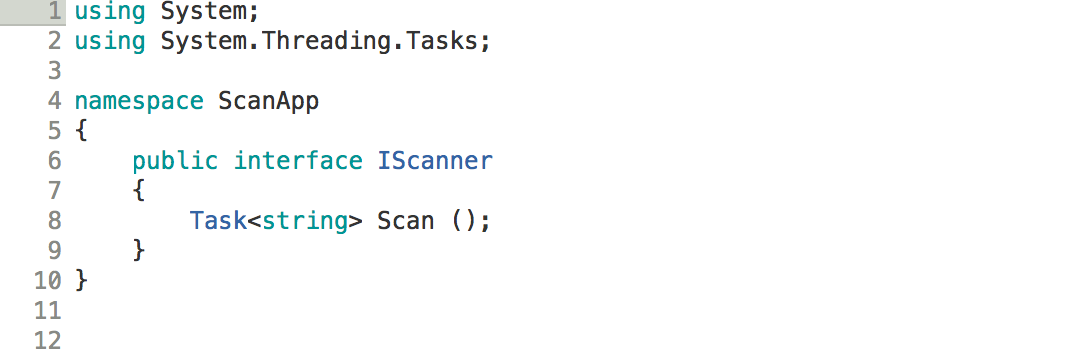
\includegraphics[scale = 0.4]{graphics/IScanner.png}
\caption{Das Interface IScanner}
\label{fig:abb28}
\end{figure}
\subsection{Web Services f�r die Kommunikation mit dem Backend}